\documentclass[journal]{IEEEtran}
\usepackage[a5paper, margin=10mm, onecolumn]{geometry}
\usepackage{lmodern} % Ensure lmodern is loaded for pdflatex
\usepackage{tfrupee} % Include tfrupee package

\setlength{\headheight}{1cm} % Set the height of the header box
\setlength{\headsep}{0mm}     % Set the distance between the header box and the top of the text

\usepackage{gvv-book}
\usepackage{gvv}
\usepackage{cite}
\usepackage{amsmath,amssymb,amsfonts,amsthm}
\usepackage{algorithmic}
\usepackage{graphicx}
\usepackage{textcomp}
\usepackage{xcolor}
\usepackage{txfonts}
\usepackage{listings}
\usepackage{enumitem}
\usepackage{mathtools}
\usepackage{gensymb}
\usepackage{comment}
\usepackage[breaklinks=true]{hyperref}
\usepackage{tkz-euclide} 
\usepackage{listings}                                      
\def\inputGnumericTable{}                                 
\usepackage[latin1]{inputenc}                                
\usepackage{color}                                            
\usepackage{array}                                            
\usepackage{longtable}
\usepackage{multicol}
\usepackage{calc}                                             
\usepackage{multirow}                                         
\usepackage{hhline}                                           
\usepackage{ifthen}                                           
\usepackage{lscape}
\begin{document}

\bibliographystyle{IEEEtran}
\vspace{3cm}

\title{9.3.11.1}
\author{EE24BTECH11042 - M.SRUJANA}
{\let\newpage\relax\maketitle}

\renewcommand{\thefigure}{\theenumi}
\renewcommand{\thetable}{\theenumi}
\setlength{\intextsep}{10pt} % Space between text and floats


\numberwithin{equation}{enumi}
\numberwithin{figure}{enumi}
\renewcommand{\thetable}{\theenumi}


\textbf{Question}:\newline
Solve the differential equation $\frac{d^2y}{dx^2} = -y$ with initial conditions $y(0) = 1$ and $y'(0) = 0$
\newline
\textbf{Solution: }
\newline
Theoretical Solution:\\
Laplace Transform definition\\
\begin{align}
	\mathcal{L}(f(t)) = \int_{0}^{\infty} e^{-st} f(t) dt
\end{align}
Properties of Laplace Transform:
\begin{align}
	\mathcal{L}(y'') &= s^2 \mathcal{L}(y) - s y(0) - y'(0) \\
	\mathcal{L}(1) &= \frac{1}{s} \\
	\mathcal{L}(cf(t)) &= c \mathcal{L}(f(t)) \\
	\mathcal{L}(e^{at} f(t)) &= F(s-a)
\end{align}
Applying the Laplace Transform to the differential equation:
\begin{align}
	y'' + y &= 0 \\
	\mathcal{L}(y'') + \mathcal{L}(y) &= 0 \\
	s^2 \mathcal{L}(y) - s y(0) - y'(0) + \mathcal{L}(y) &= 0
\end{align}
Substitute the initial conditions:
\begin{align}
	(s^2 + 1)\mathcal{L}(y) &= s \\
	\mathcal{L}(y) &= \frac{s}{s^2 + 1} \\
	\mathcal{L}(y) &= \frac{1}{2}\left(\frac{1}{s + i} + \frac{1}{s - i}\right)
\end{align}
Taking the inverse Laplace transform:
\begin{align}
	y &= \frac{1}{2}\left( e^{ix} + e^{-ix} \right) \\
	y &= \cos(x)
\end{align}
So, the theoretical solution is:
\begin{align}
	y(x) = \cos(x)
\end{align}

Now, we will find the difference equation using the Bilinear Z-transform.

Using the substitution for \( s \):
\begin{align}
	s &= \frac{2}{T}\left( \frac{1 - z^{-1}}{1 + z^{-1}} \right)
\end{align}
Applying this substitution to the Laplace transform expression:
\begin{align}
	Y(z) &= \frac{1}{2} \left( \frac{T(1 + z^{-1})}{2(1 - z^{-1}) + T(1 + z^{-1})} + \frac{T(1 + z^{-1})}{2(1 - z^{-1}) - T(1 + z^{-1})} \right)
\end{align}
Simplify the expression:
\begin{align}
	Y(z) &= \frac{T(1 + z^{-1})}{2(1 - z^{-1}) + T(1 + z^{-1})} - \frac{T(1 + z^{-1})}{2(1 - z^{-1}) - T(1 + z^{-1})}
\end{align}
Define the constants:
\begin{align}
	\alpha_1 &= -\frac{T - 2}{T + 2} \\
	\alpha_2 &= -\frac{T + 2}{T - 2}
\end{align}
Thus, we have:
\begin{align}
	Y(z) = \frac{T}{2(T + 2)} \left( \frac{1}{1 - \alpha_1 z^{-1}} + \frac{z^{-1}}{1 - \alpha_1 z^{-1}} \right) - \frac{T}{2(T - 2)} \left( \frac{1}{1 - \alpha_2 z^{-1}} + \frac{z^{-1}}{1 - \alpha_2 z^{-1}} \right)
\end{align}

The radius of convergence is given by:
\begin{align}
	\text{Radius of convergence} = \max(\lvert \alpha_1 \rvert, \lvert \alpha_2 \rvert)
\end{align}

Finally, apply the inverse Z-transform:
\begin{align}
	(1 - \alpha_1 z^{-1})(1 - \alpha_2 z^{-1}) Y(z) &= \frac{T}{2} \left( \frac{1 - (\alpha_2 - 1) z^{-1} - \alpha_2 z^{-2}}{T + 2} - \frac{1 - (\alpha_1 - 1) z^{-1} - \alpha_1 z^{-2}}{T - 2} \right)
\end{align}

Rearrange to get the difference equation:
\begin{align}
	y_{n+2} - (\alpha_1 + \alpha_2) y_{n+1} + y_n = \frac{T}{2} \left( \frac{\alpha_1}{T - 2} - \frac{\alpha_2}{T + 2} \right) \delta(n)
\end{align}

Now, moving to the computational solution, discretize the equation using the trapezoidal rule:
\begin{align}
	y_{k+1} - y_{k} &= \frac{h}{2} \left( y'_{k} + y'_{ k+1} \right) \\
	y'_{k+1} - y'_{k} &= \frac{h}{2} \left( y_{k} + y_{ k+1} \right)
\end{align}
Solve for \( y_{k+1} \) and \( y'_{k+1} \):
\begin{align}
	y_{k+1} = \frac{(y_{k})(4 + h^2) + 4h y'_{k}}{4 - h^2} \\
	y'_{k+1} = \frac{(y'_{k})(4 + h^2) + 4h y_{k}}{4 - h^2}
\end{align}

Use these difference equations to compute the values of \( y \) and \( y' \) at each step and plot the results. The figure below compares the theoretical and computational solutions.\\
Comparison between the theoretical solution and computational solutions.

\begin{figure}[h!]
   \centering
   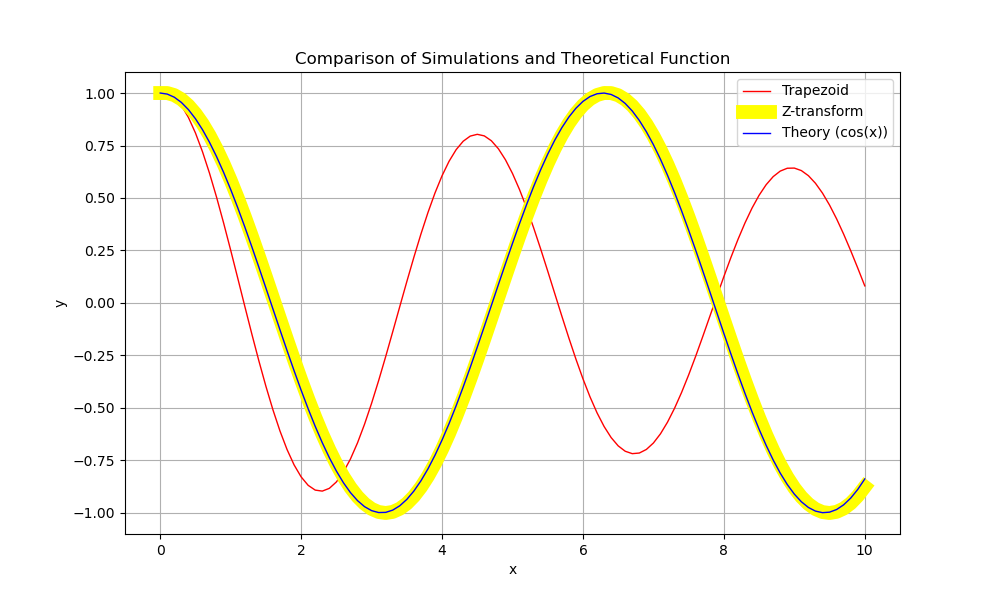
\includegraphics[width=\columnwidth]{fig/fig.png}
\end{figure}



\end{document}

